\newcommand{\neuron}[3]{\draw[fill, white] (#1, #2) circle (0.5); \draw (#1, #2) circle (0.5) node {#3};}

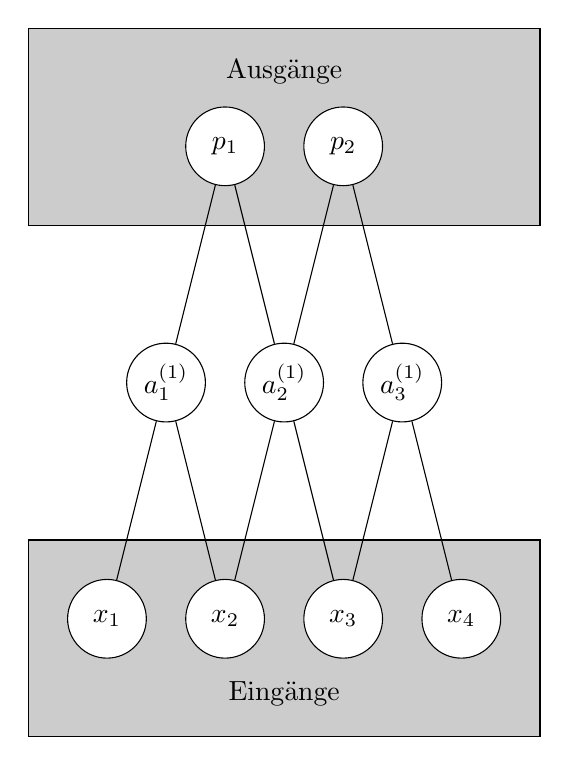
\begin{tikzpicture}
	\draw[fill=black!20] (-1, -1.5) rectangle (5.5, 1) node[midway, yshift=-20] {Eingänge};
	\draw[fill=black!20] (-1, 5) rectangle (5.5, 7.5) node[midway, yshift=20] {Ausgänge};

	% Verbindungen
	\draw (0, 0) -- (0.75 + 0, 3);
	\draw (1.5, 0) -- (0.75 + 0, 3);
	\draw (1.5, 0) -- (0.75 + 1.5, 3);
	\draw (3, 0) -- (0.75 + 1.5, 3);
	\draw (3, 0) -- (0.75 + 3, 3);
	\draw (4.5, 0) -- (0.75 + 3, 3);
	
	\draw (0.75 + 0, 3) -- (1.5, 6);
	\draw (0.75 + 1.5, 3) -- (1.5, 6);
	
	\draw (0.75 + 1.5, 3) -- (3, 6);
	\draw (0.75 + 3.0, 3) -- (3, 6);
	
	% Eingänge
	\neuron{0}{0}{$x_1$}
	\neuron{1.5}{0}{$x_2$}
	\neuron{3}{0}{$x_3$}
	\neuron{4.5}{0}{$x_4$}
	
	% 1. Layer
	\neuron{0.75 + 0}{3}{$a_1^{(1)}$}
	\neuron{0.75 + 1.5}{3}{$a_2^{(1)}$}
	\neuron{0.75 + 3}{3}{$a_3^{(1)}$}
	
	% Ausgänge
	\neuron{1.5 + 0}{6}{$p_1$}
	\neuron{1.5 + 1.5}{6}{$p_2$}
\end{tikzpicture}